\section{Domain Model}
\label{sec:domainmodel}

\begin{figure}[h]
\center
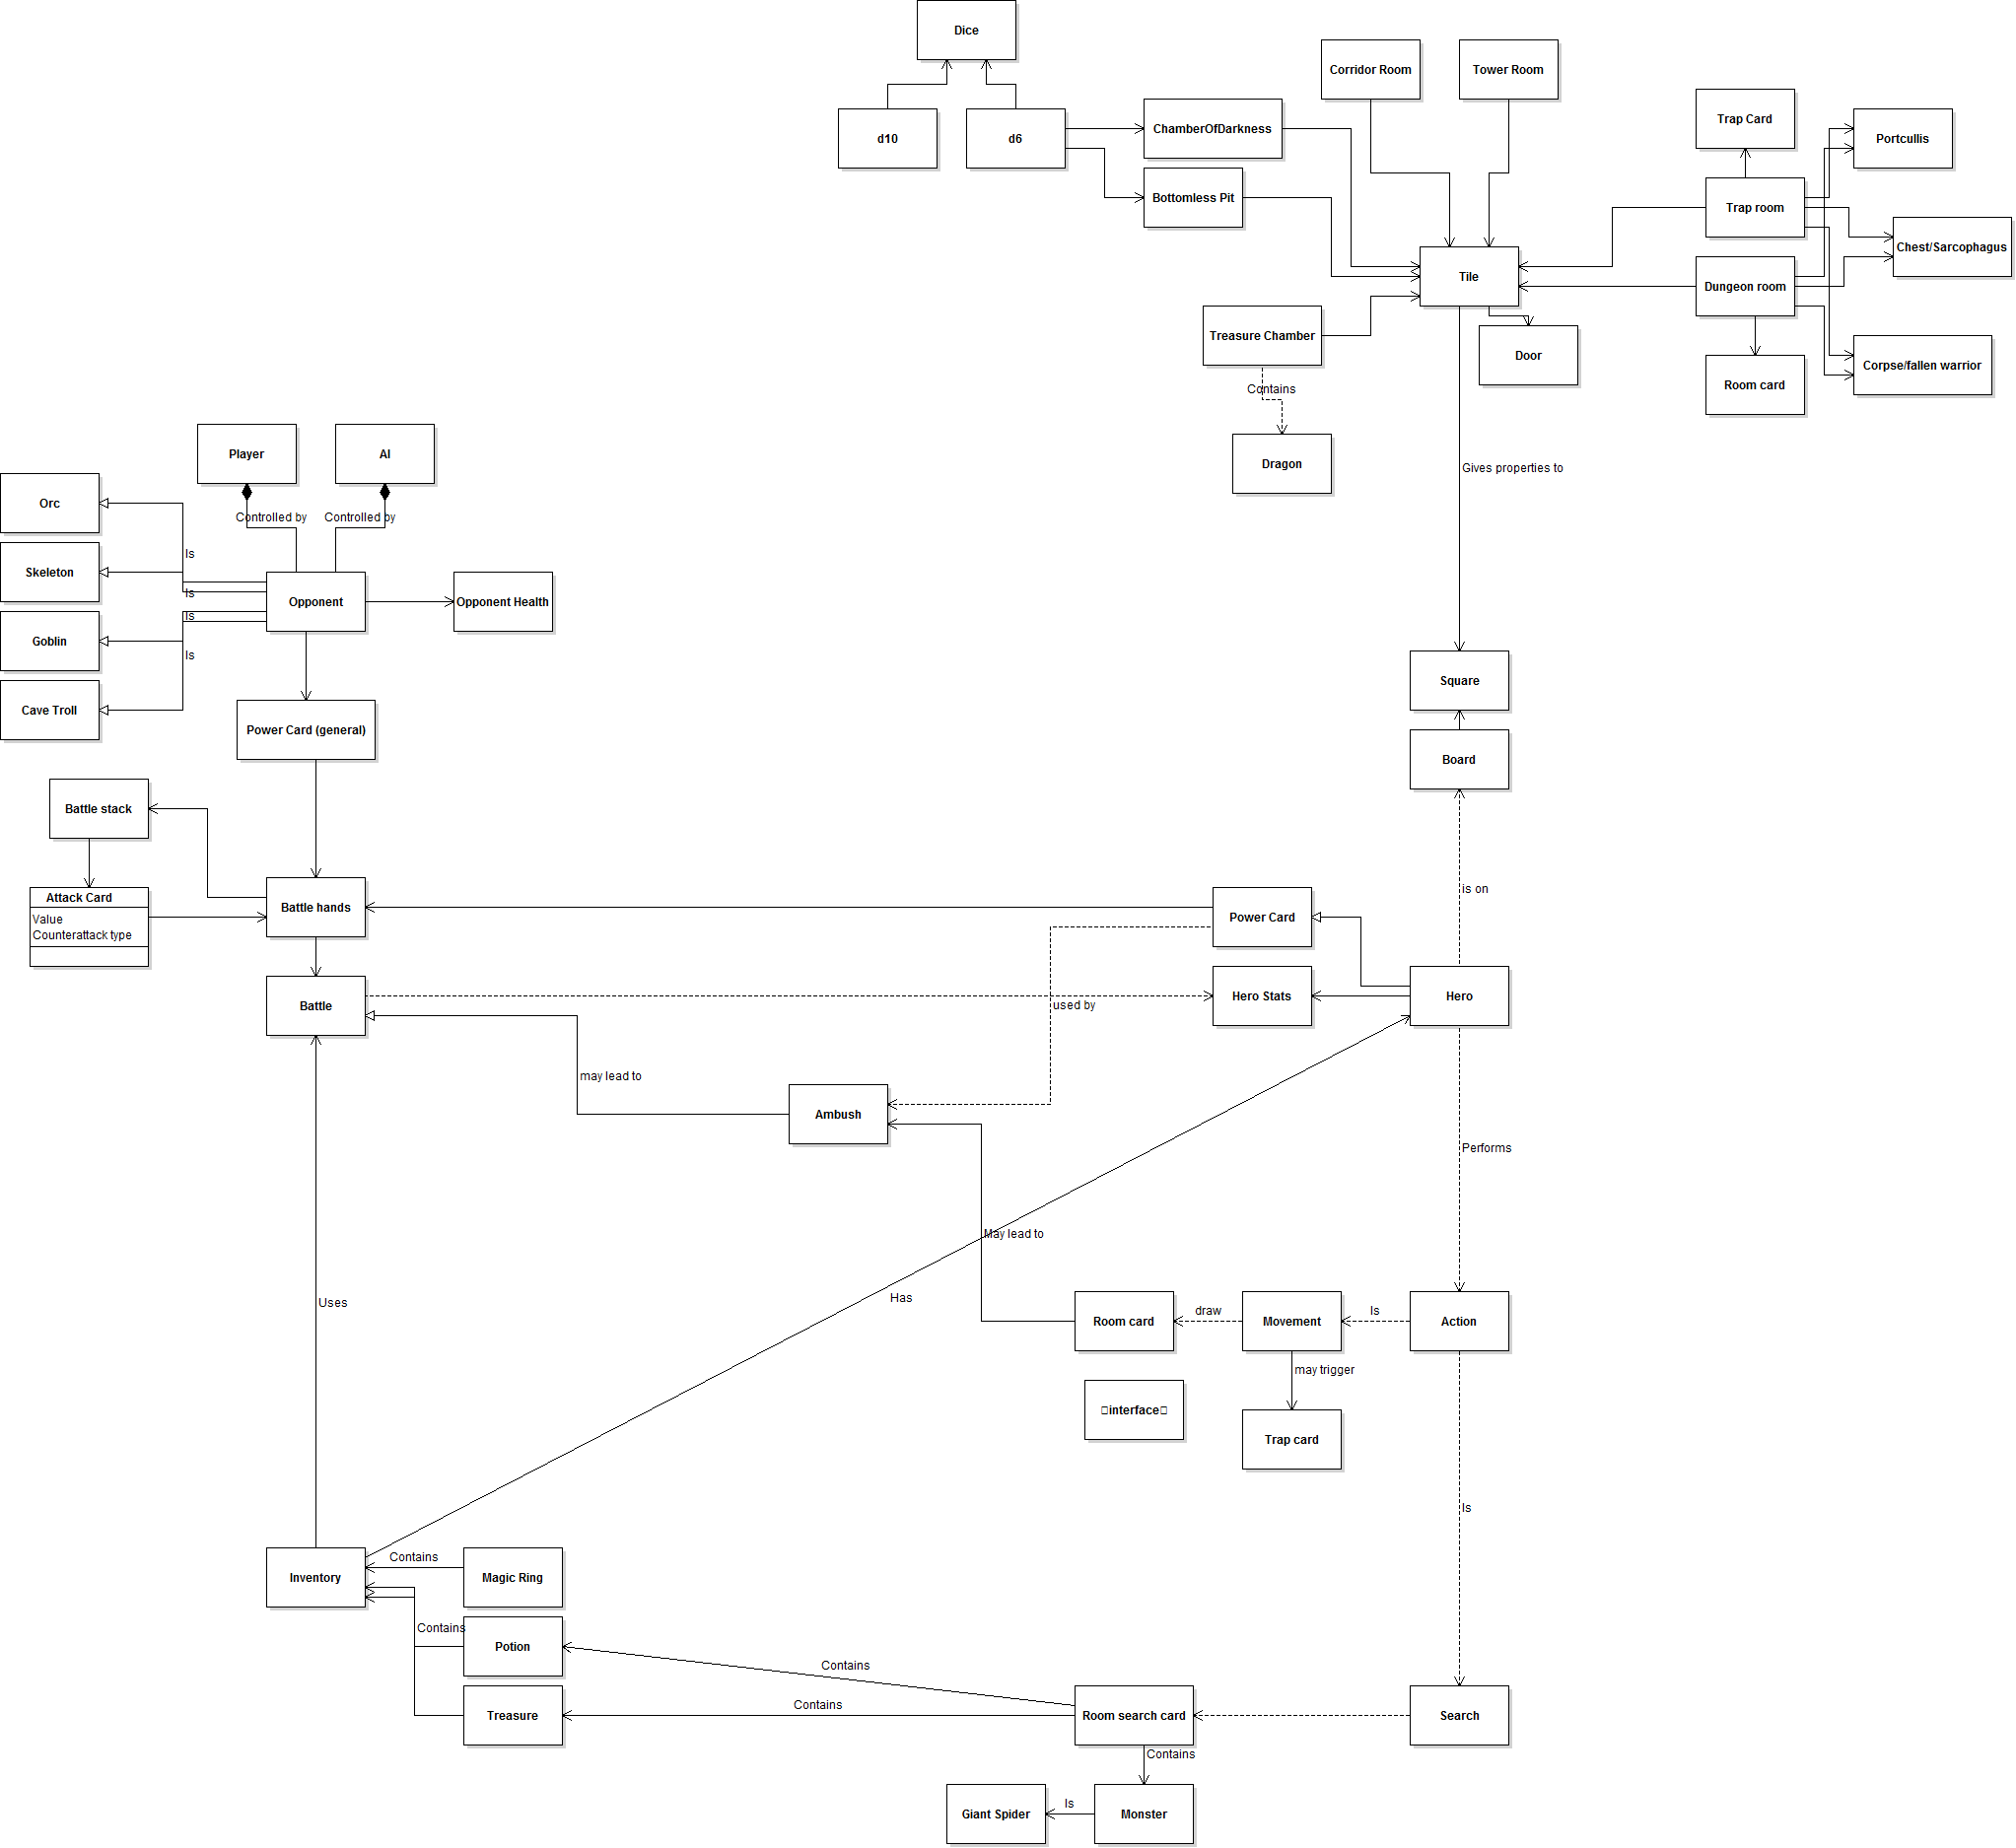
\includegraphics[width=\textwidth]{diagrams/DomainModel.png}
\caption{The domain model for the game. The arrows may be misleading as the relation sometimes goes in both directions, so use caution when interpreting them.}
\label{fig:domain_model}
\end{figure}

The Domain Model is an analysis artifacts that helps the designer create an understanding of the objects and concepts used in the game the software will model. It visualizes how objects relate to each other and gives the designer a better understanding of the elements of the game. By reading through the game rules and description we can extract a set of nouns used within the game, and place them as objects in our model, together with the interactions between the objects. This is a great help when deciding which objects belong together and may make up a subsystem in the software implementation. The domain model for the DragonQuest game is displayed in Figure \ref{fig:domain_model}.

From the domain model it is immediately clear that the game board (\textsc{Board}) and the objects associated with it is a clear candidate for a subsystem, as is the battling part of the game. This modularity is transferred to the class diagram, presented in Section \ref{sec:staticdiagrams}.

